\section{La creazione del server principale}

Per poter essere in grado di gestire un numero elevato di richieste in tempi ridotti, l’applicazione deve garantire un’elevata scalabilità.\\
\\
Capace di soddisfare al meglio questa esigenza è Azure Functions, un servizio serverless che consente di suddividere il codice in unità indipendenti,
ciascuna eseguita in un ambiente di esecuzione unico per ogni richiesta.
Questa caratteristica, combinata con la virtualizzazione dell’ambiente di esecuzione offerta dal cloud, consente una scalabilità potenzialmente illimitata.\\
\\
L’indipendenza e la natura stateless di ogni funzione, ovvero la sua esecuzione svincolata dalle informazioni sullo stato o sulla sessione, sono responsabilità dello sviluppatore.
Ogni funzione segue il principio di singola responsabilità, eseguendo un unico compito specifico.
Tuttavia, nel caso di richieste che necessitino l’esecuzione coordinata di più funzioni, Azure Durable Functions fornisce una soluzione efficace.\\
\\
Integrata all’interno delle Azure Functions, Azure Durable Function consente la creazione di una funzione orchestrator,
incaricata di gestire l’ordine, lo stato, il ciclo di vita e le risposte delle varie funzioni coinvolte nell’elaborazione della richiesta.\\
\\
Mantenendo un'architettura indipendente e scalabile, questa soluzione consente di gestire efficacemente scenari in cui un’esecuzione sequenziale delle operazioni è cruciale,
dove è necessario effettuare tentativi aggiuntivi in caso di errore o fallimento o si richiede l'attesa del completamento di operazioni con un tempo di esecuzione prolungato.\\
\\
Tuttavia, l'architettura stateless e l’accoppiamento debole tra orchestrator e funzioni in esecuzione causano un tempo di risposta delle Azure Durable Functions più elevato.
Per ottimizzare l’allocazione delle risorse, il sistema avvia perciò solo le funzioni strettamente necessarie all’esecuzione del compito determinato,
stanziando al minimo il consumo computazionale.
\clearpage

\subsection{La scelta del linguaggio di programmazione}
Come linguaggio di programmazione per lo sviluppo delle funzioni è stato utilizzato C\#.
La consapevolezza che sia l’ambiente di sviluppo di C\#, ovvero il framework .Net, sia la piattaforma Azure siano entrambi sviluppati e mantenuti dalla stessa azienda, Microsoft,
garantisce elevati livelli di stabilità, supporto e coordinamento delle tecnologie adottate.\\
\\
Inoltre, l’integrazione con Entity Framework Core permette la mappatura direttamente in oggetti dei componenti del dominio, 
semplificando così la logica delle relazioni ed astraendo le comunicazioni con il database.
Grazie all’utilizzo delle proprietà virtuali degli oggetti si può applicare il lazy loading, 
riducendo il numero di richieste al database solo a quando esse sono strettamente necessarie, mantenendo in codice a livello logico ed ottimizzandone le prestazioni.\\
\\
Azure Functions in ambiente .Net supporta due modelli di esecuzione e sviluppo: in-process worker o isolated worker.
Il worker è il processo all’interno dell’applicativo che gestisce la creazione delle risorse e l’esecuzione delle funzioni in risposta alle richieste.
Nella modalità in-process, la funzione viene eseguita all’interno dello stesso processo del worker che l’ha generata,
riducendo la quantità di allocazione delle risorse necessarie ma condividendo l’ambiente di esecuzione.
Nel modello isolated, invece, ogni funzione viene eseguita attraverso un processo indipendente dedicato,
garantendo maggiore isolamento e quindi riducendo le possibili dipendenze tra le funzioni. \\
\\
Inoltre, il modello isolated worker offre ulteriori vantaggio grazie al maggiore supporto fornito:
innanzitutto esso prevede una maggiore compatibilità, grazie al più ampio numero di versioni del framework .Net a disposizione,
a differenza del modello in-process, limitato alle sole versioni con supporto a lungo termine.
In secondo luogo, il supporto per la creazione di middleware personalizzati 
permette l’elaborazione di un codice intermedio tra la chiamata e l’esecuzione della funzione,
funzionalità invece non disponibile nel modello in process.
Considerati questi vantaggi, le funzioni sono state sviluppate utilizzando il modello isolated worker 
per garantire maggiore flessibilità, compatibilità e modularità dell’architettura.
\clearpage


\subsection{L'implementazione della logica applicativa}
Per quanto ogni funzione ricopra un unico compito, alcuni parti possono dover essere condivise.
Per questo motivo, la logica applicativa è stata suddivisa creando un metono specifico per ogni singola esigenza,
che le funzioni chiameranno ogni volta che ne hanno bisogno.
I metodi vengono quindi raggruppati in classi in base all'inerenza dei loro scopi, 
concentrando il codice che condivide le stesse necessità e uniformando il suo stile.
Le dipendenze vengono quindi inizializzate un'unica volta a livello di classe, creando un software più ordinato.\\
\\
Nella stessa modalità di suddivisione delle responsabilità del client, 
le classi sono state sviluppate tenendo conto delle divisioni del dominio e di ulteriori responsabilità specifiche. 
Per ogni elemento principale del dominio è stata sviluppata una classe service che implementa le operazioni relative,
mentre, per compiti che richiedono particolare attenzione o che astraggono l'interazione con una particolare risorsa, 
vengono implementate classi apposite.\\
\\
Ogni servizio relativo agli elementi strutturali ha bisogno di una connessione con il database per poter applicare le modifiche eseguite.
Questa viene implementata da una classe chiamata WydDbContext che racchiude la logica 
e le impostazioni legate alla persistenza principale.
Si concentrano così in un'unico luogo tutte le necessità e le configurazioni di basso livello relative alla sua interazione,
quali la definizione del dominio e delle sue relazioni ed 
eventuali operazioni da applicare in automatico qualora la natura dell'oggetto lo richieda.
Ad esempio, alcune classi richiedono l'aggiornamento automatico della data di ultima modifica.
L'implementazioni delle classi del dominio viene trattata nei capitoli seguenti.\\
\\
Per alcuni compiti specifici sono state implementate classi apposite.
In particolare, AuthorizationService si occupa dell'autenticazione e dell'autorizzazione della richiesta,
mentre NotificationService astrae la relazione con il servizio di aggiornamento in tempo reale.
\clearpage
\begin{figure}[h!]
    \begin{center}
        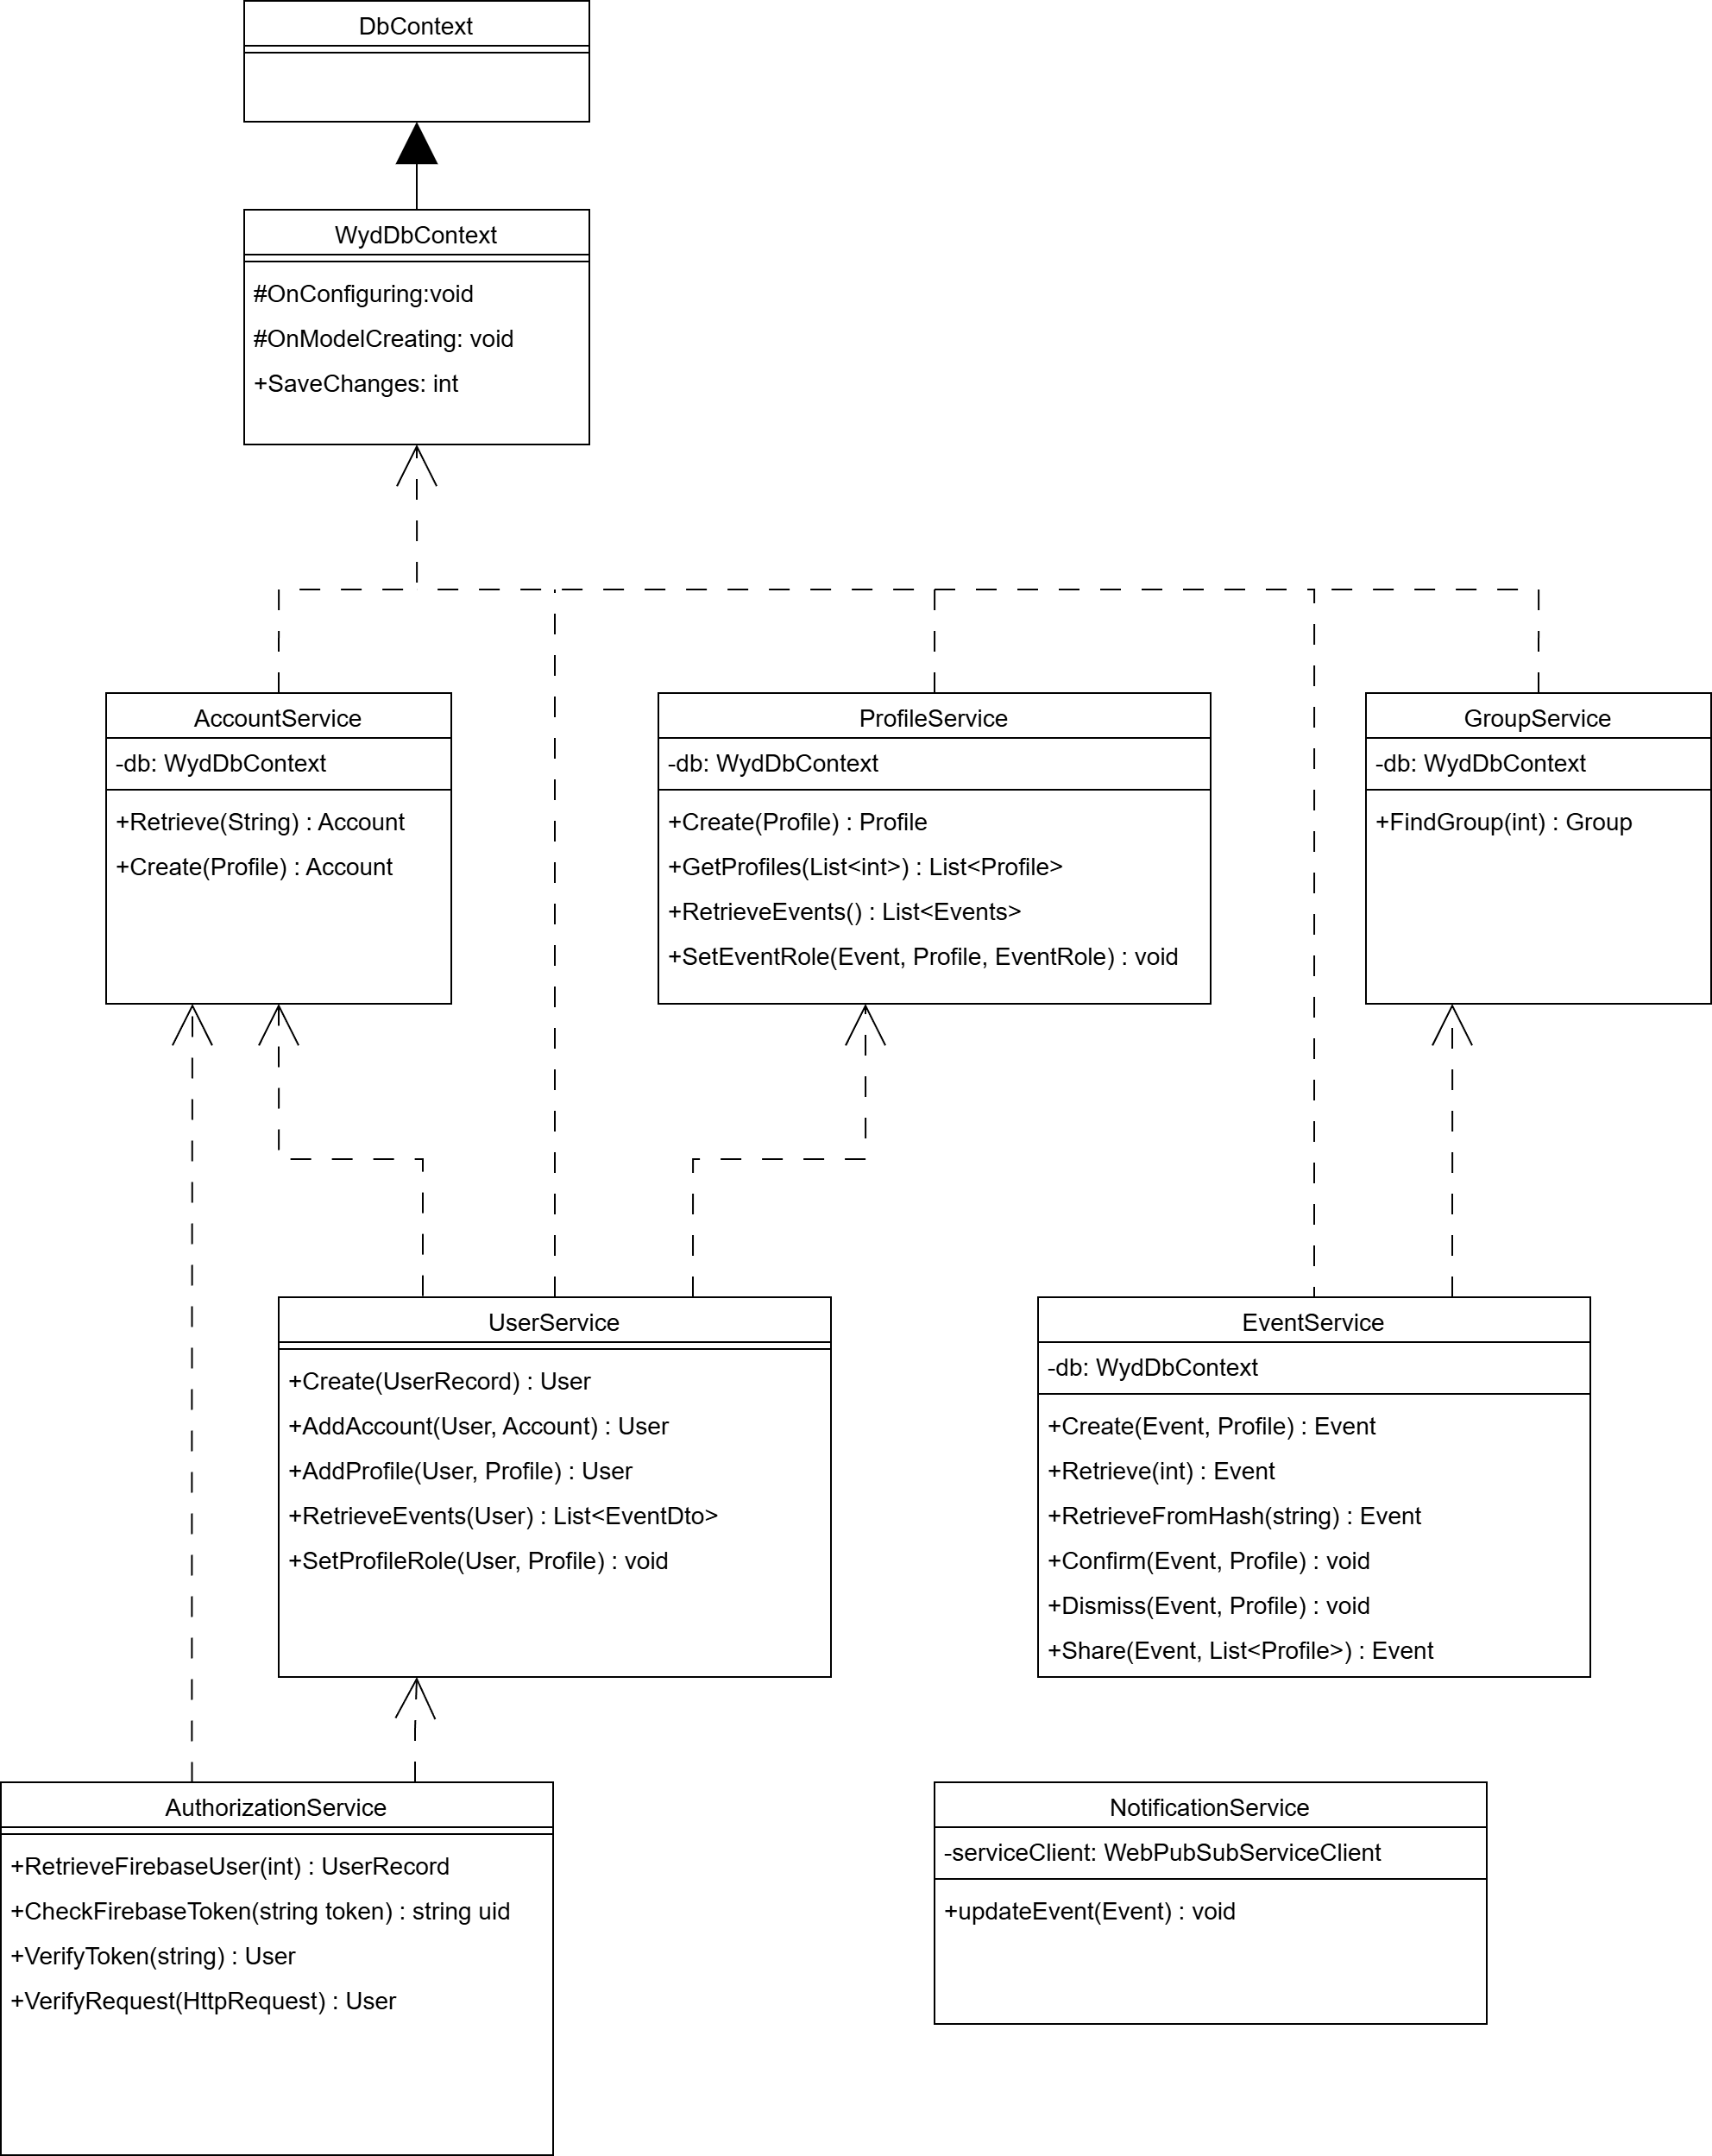
\includegraphics[width=\textwidth]{ServiceClassDiagram.png}
        \caption{Modello delle classi del server}
    \end{center}
\end{figure}
\clearpage
\begin{figure}[h!]
    \begin{center}
        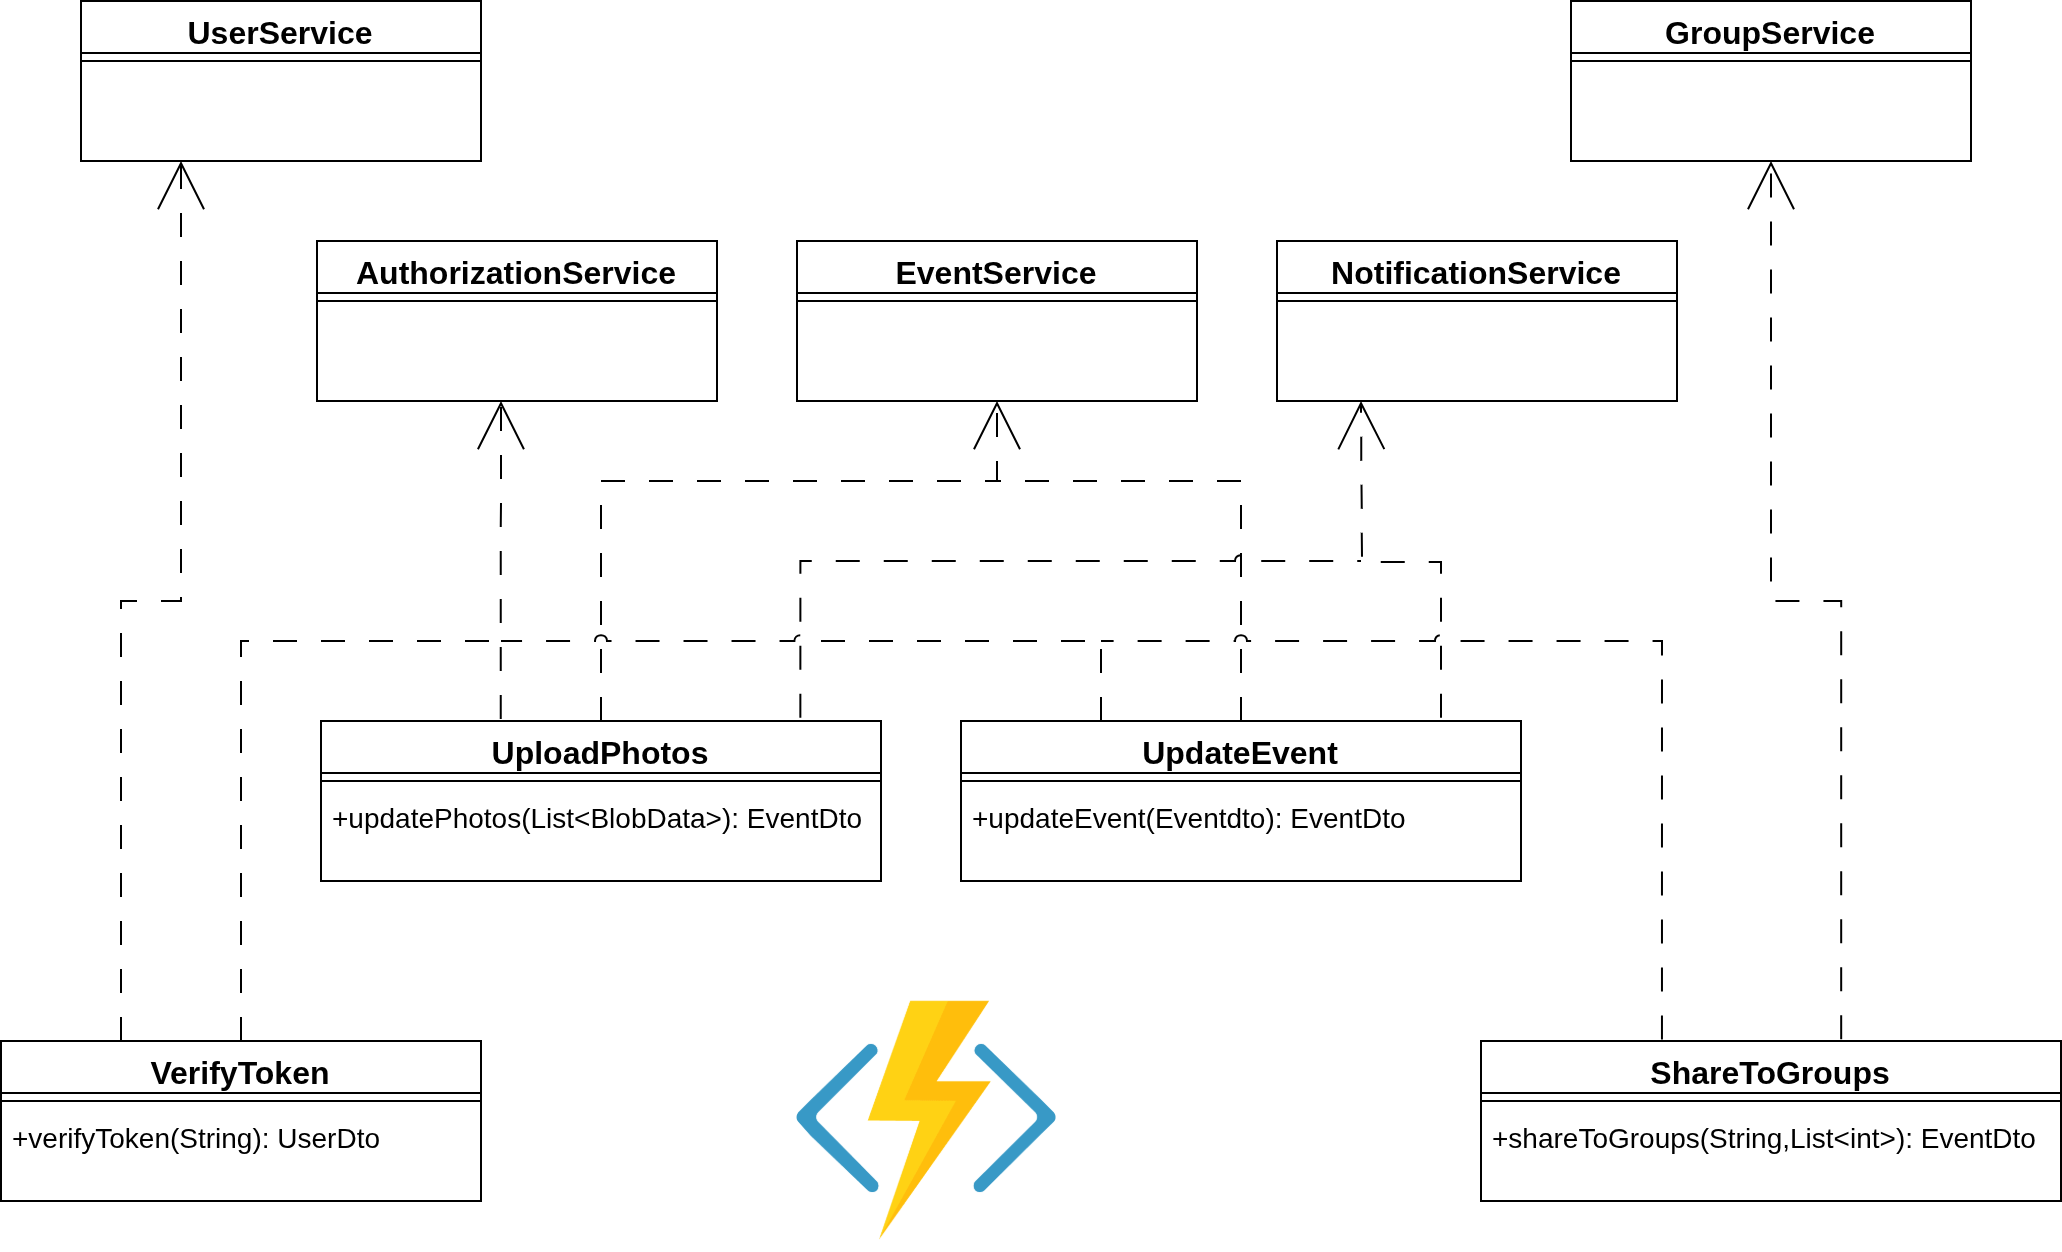
\includegraphics[width=\textwidth]{FunctionClassDiagram.png}
        \caption{Modello delle relazioni tra Functions e i servizi usati}
    \end{center}
\end{figure}
Per allineare i dati a disposizione del server con il dominio del client
e per ridurre l'invio delle informazioni non necessarie, sono stati creati dei Data Transfer Object(DTO).
I DTO sono classi logiche che prevedono almeno un costruttore che, dato l'elemento del dominio, 
ne copia solo le informazioni necessarie. 
Questo permette di creare rappresentazioni dei dati come necessarie al client,
mascherando le logiche applicative e di fatto separando le dipendenze del dominio dai requisiti di comunicazione.\\
\\
\begin{figure}[h!]
    \begin{center}
        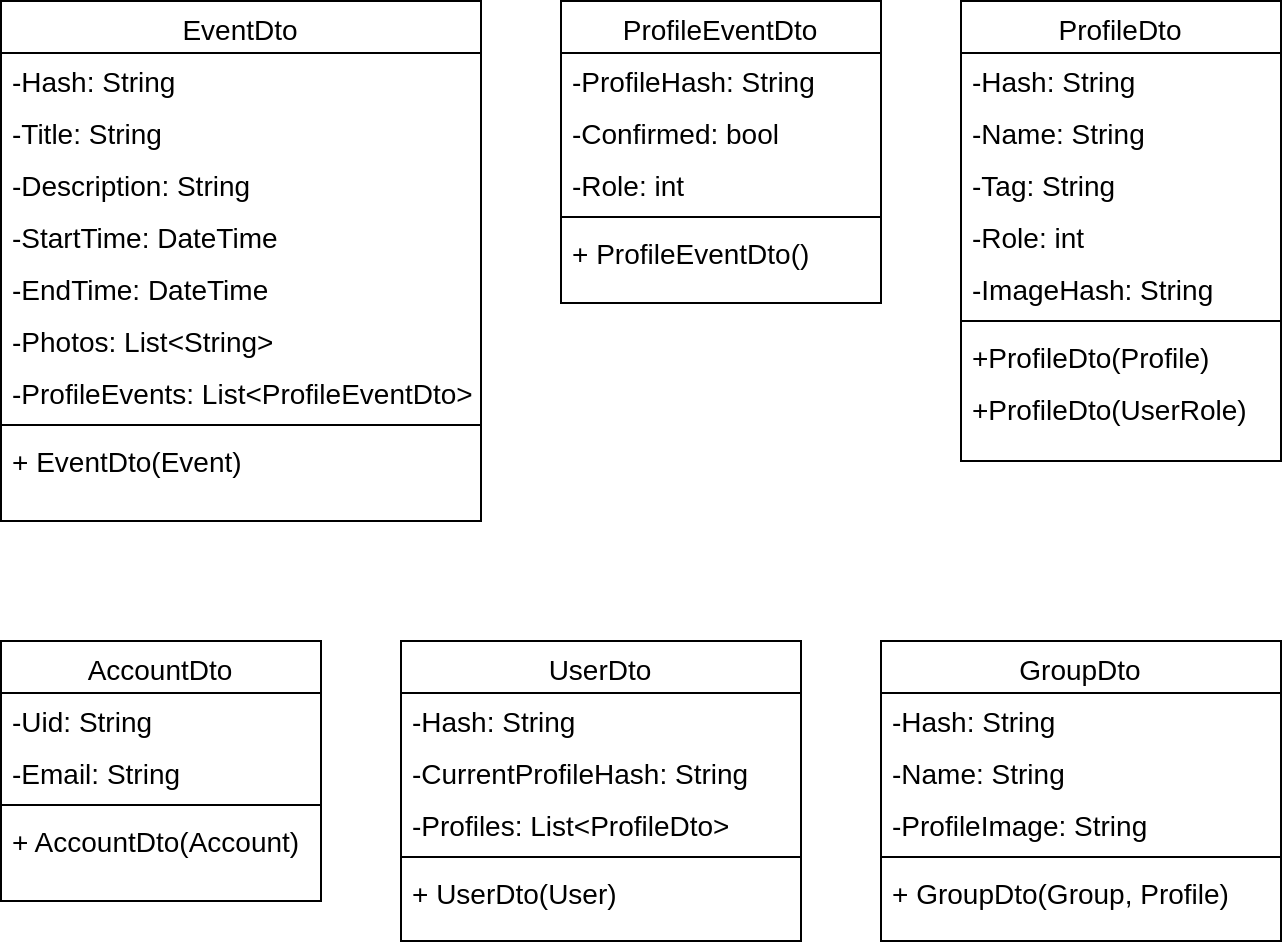
\includegraphics[height=0.41\textheight]{DTOClassDiagram.png}
        \caption{Modello delle classi dei data tranfer object}
    \end{center}
\end{figure}
\clearpage
Per ogni metodo pubblico delle classi service sono stati implementati dei test.
I test permettono la simulazione di differenti situazioni per controllare che il codice segua il comportamento desiderato.
La loro implementazione è quindi precedente allo sviluppo stesso delle classi, 
in quanto le aspettative sono già note, e il superamento dei test determina la correttezza del metodo.
Inoltre, in caso di necessità particolari che escono dalle normali aspettative della funzione, 
quali, ad esempio, il controllo di un valore particolare o l'implementazione di un vincolo specifico,
i test assicurano la loro futura presa in carico anche in caso di modifica totale del codice.
\begin{figure}[h!]
    \begin{center}
        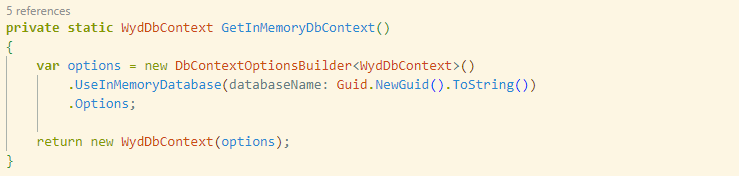
\includegraphics[width=\textwidth]{TestInit.png}
        \caption{Simulazione del database}
    \end{center}
\end{figure}

\begin{figure}[h!]
    \begin{center}
        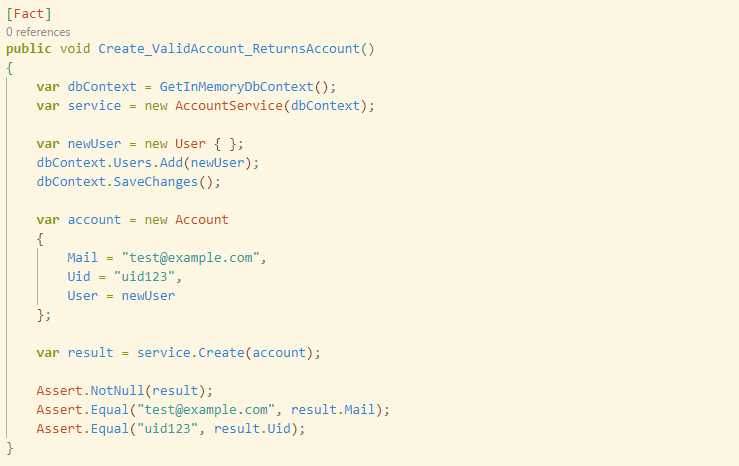
\includegraphics[width=\textwidth]{TestAccount2.png}
        \caption{Test di creazione di un account}
    \end{center}
\end{figure}

\clearpage

\subsection{La modalità di distribuzione e aggiornamento}
Lo sviluppo è stato condotto utilizzando Visual Studio Code, 
programma sviluppato dalla stessa Microsoft per la creazione di codice.
Visual Studio Code permette l'integrazione con molteplici estensioni fornendo il supporto
per la maggior parte delle tecnologie.\\
\\
In particolare, grazie alle estensioni dedicate al provider Azure, 
è possibile collegare il proprio ambiente di lavoro con i servizi in cloud.
Il legame così creato consente un aggiornamento immediato ed intuitivo del codice, 
gestito interamente dal programma.\\
\\
\begin{figure}[h!]
    \begin{center}
        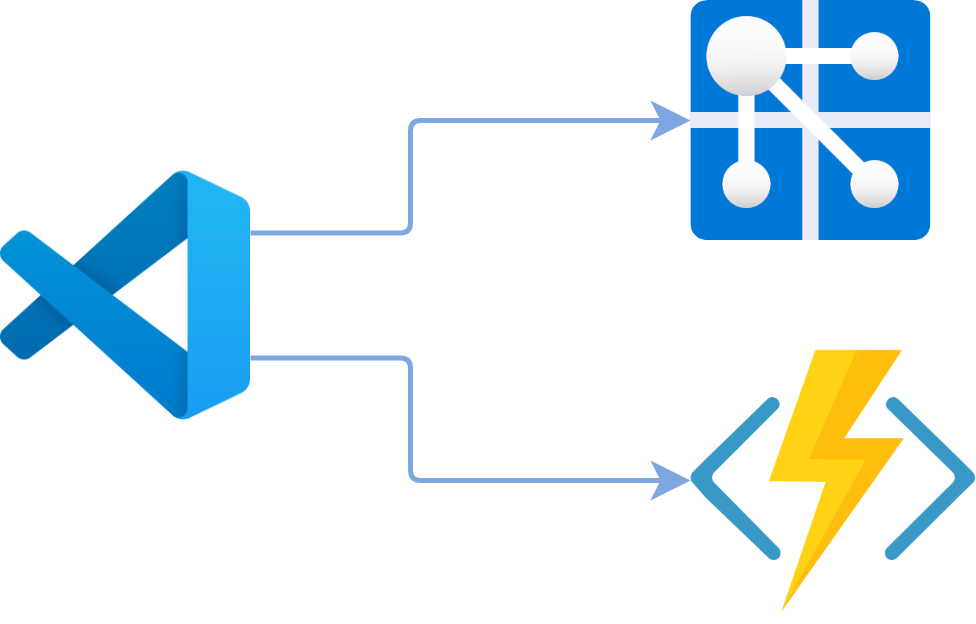
\includegraphics[height=0.25\textheight]{DeployBack.png}
        \caption{Diagramma di aggiornamento e distribuzione del server}
    \end{center}
\end{figure}

\clearpage

